Da die exakte Berechnung einer Kollision signifikant viel Rechenleistung benötigt, ist eine Vorfilterung sinnvoll. Diese schließt einen Großteil der Objektpaare schon vorher aus. Eine Kollision kann z.B. nur dann passieren, wenn die Hüllobjekte der beiden Objekte ebenfalls kollidieren (wegen der Eigenschaft //TODO mathe). Hier wird als Hüllobjekt eine AABB verwendet. Bestimmte Arten der logischen Kollision benötigen außerdem keine genauere Berechnung, sodass die verbleibenden Objektpaare nach der Vorfilterung direkt eine logische Kollision eingehen. Um verschiedene Arten der Kollision behandeln zu können und die Objektpaare dem richtigen Algorithmus für die nächste Stufe zuführen zu können, wurde im Rahmen des Projekts eine Komponente erstellt, die dieses Problem mit austauschbarem Vorfilterungsalgorithmus löst. (Ungenügende Ansätze der Behandlung verschiedener Kollisionstypen unter Verwendung eines nicht austauschbaren Vorfilterungsalgorithmus haben schon vor dem Projektstart in der Codebasis existiert). \\
Logische und physikalische Kollisionen werden als (lokale) Interaktionen zusammengefasst und werden in 2 Kategorien eingeteilt:
//TODO format
1. Symmetrische Interaktionen: Beide Objekte des Objektpaares gehören der selben Klasse an (z.B: die Kollision rigider Objekte, wie sie in //TODO ref beschrieben wird).
2. Asymmetrische Interaktionen: Objektpaare setzen sich aus 2 Objekten verschiedener Klassen zusammen (z.B. Projektil und treffbares Objekt). Kollisionen innerhalb des selben Objekts treten hier nicht auf (Projektile interagieen nicht mit anderen Projektilen).

In jeder Kategorie können mehrere Interaktionstypen enthalten sein. Jeder Typ wird hier einzeln betrachtet und ihm kann so ein eigener Vorfilterungsalgorithmus zugewiesen werden, der entsprechend zugeschnitten und problemspezifisch optimiert werden kann.
Die Aufgabe des Vorfilterungsalgorithmus unterscheidet sich je nach Kategorie der Interaktion etwas:
//TODO format
1. Symmetrische Interaktionen: Aus Menge aus n Objekten werden alle diejenigen (maximal n²) Objektpaare ausgewählt, deren AABBs sich überschneiden. Als untere Schranke kann man Omega(n+i) angeben, wobei i die Anzahl der tatsächlichen Überschneidungen ist. Die obere Schranke O(n²) erhält man durch naives Ausprobieren jeder Kombination.
2. Asymmetrische Interaktionen: Aus 2 Mengen von n und m Objekten werden alle diejenigen Objektpaare mit jeweils einem Mitglied aus jeder Menge ausgewählt, deren AABBs sich überschneiden. Als untere Schranke kann man Omega(n+m+i) angeben. Die obere Schranke O(n*m) erhält man durch naives Ausprobieren jeder Kombination.

Für die Laufzeit bei praktischen Problemen sei angemerkt, dass die Konstante oft eben so wichtig zu betrachten ist wie die asymptotische Komplexität. \\

Im folgenden werden 2 Algorithmen, die im Rahmen des Projekts implementiert wurden, näher beschrieben.

//TODO format
1. Boxsort
//TODO

//TODO format
2. Spatial Hashing
Die Grundidee besteht hier dabei, den Raum in viele Bereiche (sog. chunks) aufzuteilen und Kollisionspaare nur innerhalb dieser Bereiche zu suchen. Sind 2 Objekte weit voneinander entfernt und somit nicht im selben chunk, ist eine Überschneidung der AABBs nicht möglich und muss deshalb auch nicht betrachtet werden. Ein Beispiel für 2 Dimensionen sieht man in Abb.~\ref{fig:spatialHashing}.

\begin{figure}
    \centering
    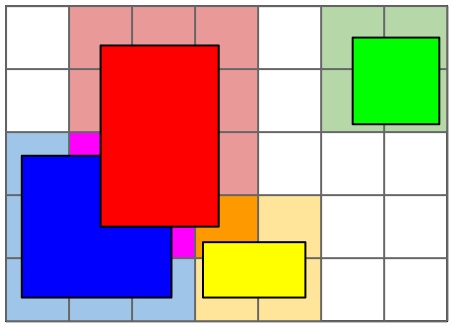
\includegraphics[width=0.5\textwidth]{./res/spatialHashingAABB.png}
    \caption{2D-Beispiel von Spatial Hashing von AABBs (stark gefärbte Rechtecke). Die leicht gefärbten Bereiche sind chunks, die ein Objekt der entsprechenden Farbe(n) beinhalten.}
    \label{fig:spatialHashing}
\end{figure}

Man sieht in Abb.~\ref{fig:spatialHashing}, dass Objekte mit mehreren chunks überlappen können. Ein Objekt muss sich in jedem chunk anmelden, das sich mit seiner AABB überschneidet, zu sehen z.B. beim grünen Objekt, das sich in den 4 chunks rechts oben anmelden muss. Gibt es keine weiteren Objekte in den chunks, wo sich das Objekt angemeldet hat, müssen keine potentiellen Kollisionen berechnet werden. Ist dies für alle Objekte der Fall, ist die optimale Komplexität O(n) im symmetrischen Fall erreicht (bei konstanter Maximalgröße von Objekten). Im asymmetrischen Fall können mehrere Objekte im selben chunk angemeldet sein, ohne dass eine Kollision auftritt, solange die Objekte alle vom selben Typ sind. In diesem Fall ist die optimale Komplexität von O(n+m) im asymmetrischen Fall erreicht (bei konstanter Maximalgröße von Objekten). \\
Werden mehrere Objekte, die für eine Kollision kompatibel sind, in einem chunk angemeldet, so müssen alle potentiellen Kollisionspaare überprüft werden (hier mit naivem //TODO Mathe O(n²) bzw. O(n*m) Algorithmus). Die Überprüfung kann entweder direkt bei der Anmeldung erfolgen (hier implementiert) oder erst nach Eintragung aller Objekte erfolgen, was die Auswahl an für die weitere Auflösung verwendbaren Algorithmen erhöht. \\
Ein potentielles Problem kann in Abb.~\ref{fig:spatialHashing} bei der Überschneidung des roten und blauen Objekts betrachtet werden. Erfolgt eine Überlappung in mehreren chunks, besteht die Gefahr der mehrfachen Behandlung von Kollisionen. Deshalb wird während der Partnerfindung ein Hashtable mit schon behandelten Objekten mitgeführt, womit effizient Duplikate vermieden werden. Auf diese Maßnahme kann verzichtet werden, wenn sich das Objekt nur in einem chunk befindet.\\
Um das Anlegen vieler leerer chunks zu vermeiden und trotzdem schnellen Zugriff zu haben, wird ein Hashtable zur Verwaltung der chunks verwendet. Dazu wurde eine passende Hashfunktion gesucht und eingebunden, die plattformunabhängig aber dennoch mit sehr geringer Laufzeit $HASH: \mathcal{I}^3 \mapsto \mathcal{I}_{64}$ mit $\mathcal{I}_{64}$ als 64-Bit Integer einem Hashwert zuordnet. $i: (i, f)\in\mathcal{S}$